% One-page architecture of the Round 3 agents (shop moss-and-oak, buyer move_76).
% Build: pdflatex architecture.tex
\documentclass[border=8pt]{standalone}
\usepackage[T1]{fontenc}
\usepackage{lmodern}
\usepackage{tikz}
\usetikzlibrary{arrows.meta,backgrounds,fit}
\definecolor{code}{HTML}{2F6B9A}
\definecolor{model}{HTML}{B5532A}
\definecolor{mem}{HTML}{3C7D4A}
\definecolor{tool}{HTML}{6B5B95}
\definecolor{mkt}{HTML}{555555}
\tikzset{
  b/.style 2 args={draw=#1, fill=#1!8, rounded corners=2pt, align=left, font=\footnotesize, inner sep=4pt, text width=#2, anchor=north west},
  a/.style={-{Stealth[length=2.2mm]}, thick, #1},
  a/.default=black!70,
  n/.style={font=\scriptsize, fill=white, inner sep=1.5pt, align=center},
}
\begin{document}
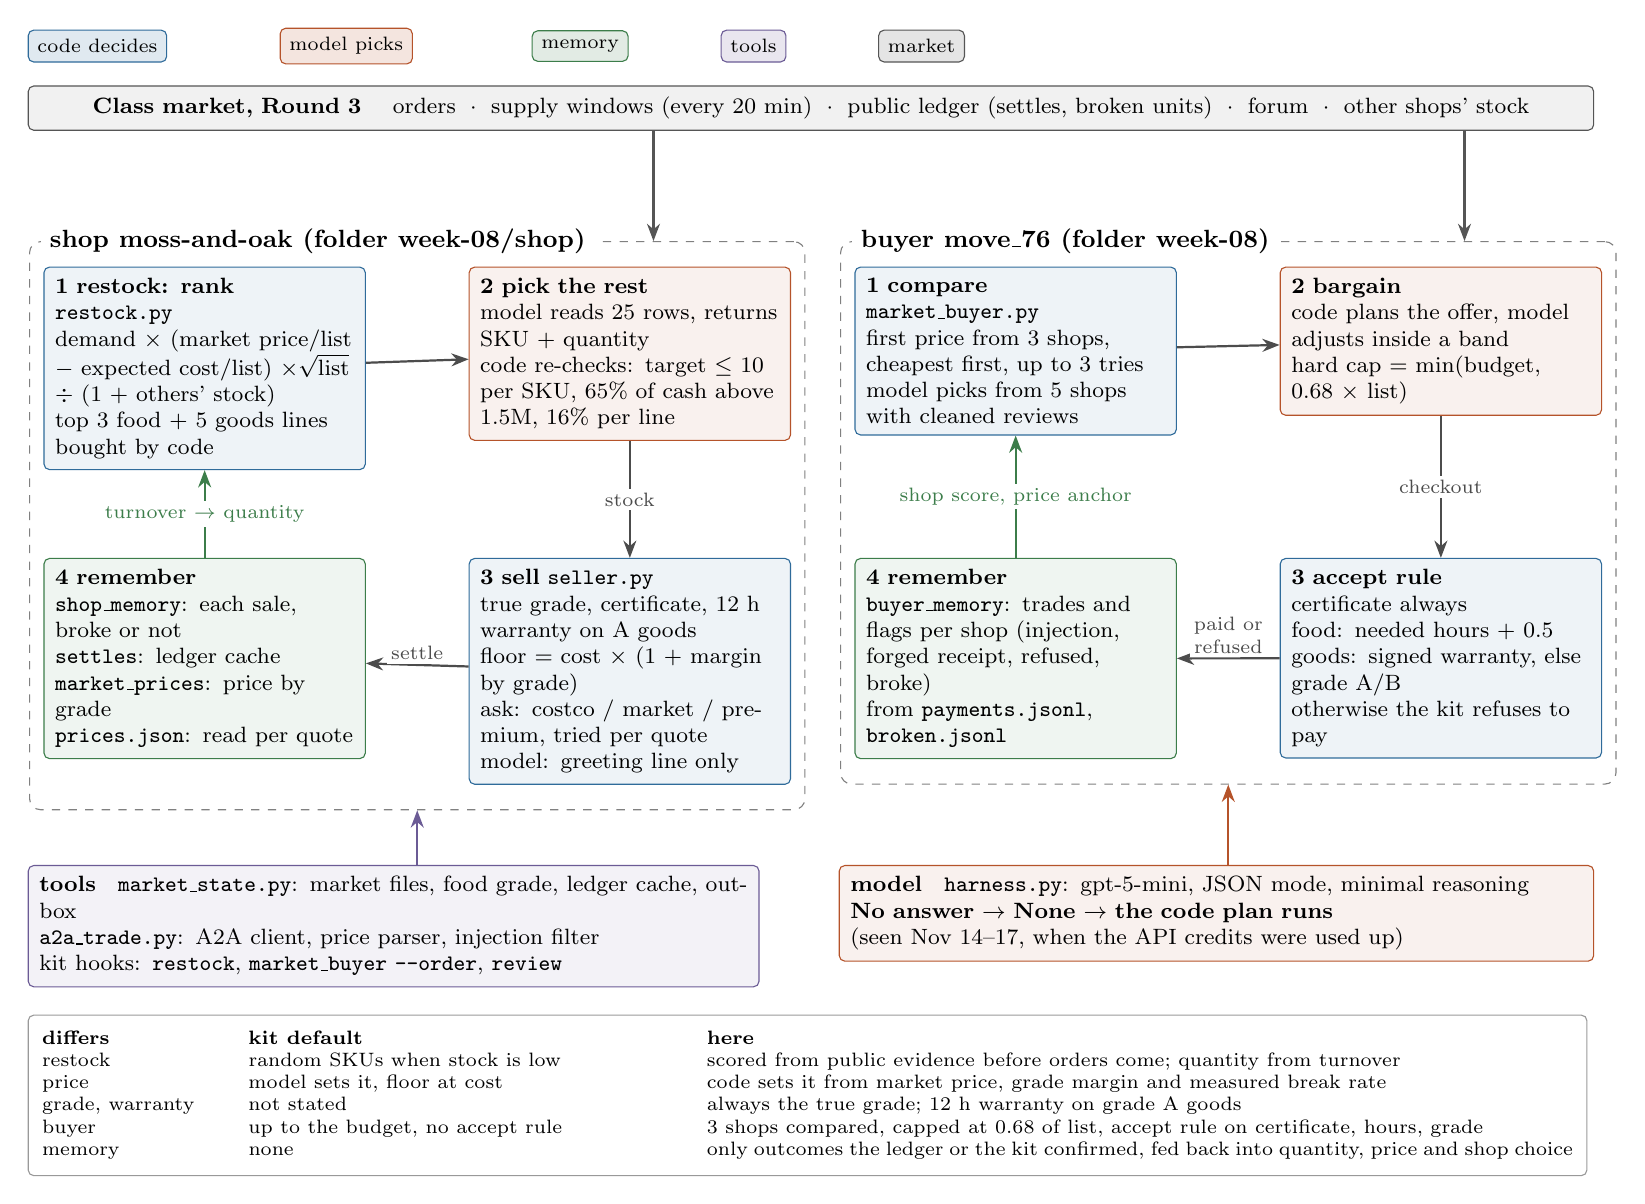
\begin{tikzpicture}[x=1cm,y=1cm]
% legend
\foreach \x/\c/\t in {0/code/code decides, 3.2/model/model picks, 6.4/mem/memory, 8.8/tool/tools, 10.8/mkt/market}
  \node[draw=\c, fill=\c!15, font=\scriptsize, rounded corners=2pt, anchor=west] at (\x,0.5) {\t};
% market
\node[b={mkt}{19.6cm}, align=center] (M) at (0,0) {\textbf{Class market, Round 3} \quad orders \;$\cdot$\; supply windows (every 20 min) \;$\cdot$\;
  public ledger (settles, broken units) \;$\cdot$\; forum \;$\cdot$\; other shops' stock};
% shop column
\node[b={code}{3.8cm}] (S1) at (0.2,-2.3) {\textbf{1 restock: rank} \texttt{restock.py}\\
  demand $\times$ (market price/list $-$ expected cost/list) $\times\sqrt{\mathrm{list}}$ $\div$ (1 + others' stock)\\
  top 3 food + 5 goods lines bought by code};
\node[b={model}{3.8cm}] (S2) at (5.6,-2.3) {\textbf{2 pick the rest}\\ model reads 25 rows, returns SKU + quantity\\
  code re-checks: target $\le$ 10 per SKU, 65\% of cash above 1.5M, 16\% per line};
\node[b={code}{3.8cm}] (S3) at (5.6,-6.0) {\textbf{3 sell} \texttt{seller.py}\\ true grade, certificate, 12 h warranty on A goods\\
  floor = cost $\times$ (1 + margin by grade)\\ ask: costco / market / premium, tried per quote\\
  model: greeting line only};
\node[b={mem}{3.8cm}] (S4) at (0.2,-6.0) {\textbf{4 remember}\\ \texttt{shop\_memory}: each sale, broke or not\\
  \texttt{settles}: ledger cache\\ \texttt{market\_prices}: price by grade\\ \texttt{prices.json}: read per quote};
\draw[a] (S1) -- (S2);
\draw[a] (S2) -- node[n]{stock} (S3);
\draw[a] (S3) -- node[n,above]{settle} (S4);
\draw[a=mem] (S4) -- node[n]{turnover $\to$ quantity} (S1);
% buyer column
\node[b={code}{3.8cm}] (B1) at (10.5,-2.3) {\textbf{1 compare} \texttt{market\_buyer.py}\\ first price from 3 shops, cheapest first, up to 3 tries\\
  model picks from 5 shops with cleaned reviews};
\node[b={model}{3.8cm}] (B2) at (15.9,-2.3) {\textbf{2 bargain}\\ code plans the offer, model adjusts inside a band\\
  hard cap = min(budget, 0.68 $\times$ list)};
\node[b={code}{3.8cm}] (B3) at (15.9,-6.0) {\textbf{3 accept rule}\\ certificate always\\ food: needed hours + 0.5\\
  goods: signed warranty, else grade A/B\\ otherwise the kit refuses to pay};
\node[b={mem}{3.8cm}] (B4) at (10.5,-6.0) {\textbf{4 remember}\\ \texttt{buyer\_memory}: trades and flags per shop (injection, forged receipt, refused, broke)\\
  from \texttt{payments.jsonl}, \texttt{broken.jsonl}};
\draw[a] (B1) -- (B2);
\draw[a] (B2) -- node[n]{checkout} (B3);
\draw[a] (B3) -- node[n,above]{paid or\\ refused} (B4);
\draw[a=mem] (B4) -- node[n]{shop score, price anchor} (B1);
\begin{scope}[on background layer]
  \node[draw=black!50, dashed, rounded corners=4pt, inner xsep=5pt, inner ysep=9pt, fit=(S1)(S2)(S3)(S4)] (SL) {};
  \node[draw=black!50, dashed, rounded corners=4pt, inner xsep=5pt, inner ysep=9pt, fit=(B1)(B2)(B3)(B4)] (BL) {};
\end{scope}
\node[font=\small\bfseries, fill=white, anchor=west] at ([xshift=4pt]SL.north west) {shop moss-and-oak (folder week-08/shop)};
\node[font=\small\bfseries, fill=white, anchor=west] at ([xshift=4pt]BL.north west) {buyer move\_76 (folder week-08)};
\draw[a=mkt] ([xshift=3cm]M.south -| SL.north) -- ([xshift=3cm]SL.north);
\draw[a=mkt] ([xshift=3cm]M.south -| BL.north) -- ([xshift=3cm]BL.north);
% shared
\node[b={tool}{9.0cm}] (T) at (0,-9.9) {\textbf{tools} \; \texttt{market\_state.py}: market files, food grade, ledger cache, outbox\\
  \texttt{a2a\_trade.py}: A2A client, price parser, injection filter\\ kit hooks: \texttt{restock}, \texttt{market\_buyer --order}, \texttt{review}};
\node[b={model}{9.3cm}] (L) at (10.3,-9.9) {\textbf{model} \; \texttt{harness.py}: gpt-5-mini, JSON mode, minimal reasoning\\
  \textbf{No answer $\to$ None $\to$ the code plan runs}\\ (seen Nov 14--17, when the API credits were used up)};
\draw[a=tool] (T.north -| SL.south) -- (SL.south);
\draw[a=model] (L.north -| BL.south) -- (BL.south);
\node[draw=black!40, rounded corners=2pt, align=left, font=\scriptsize, inner sep=5pt, anchor=north west] at (0,-11.8) {%
\begin{tabular}{@{}p{2.2cm}p{5.4cm}p{11.0cm}@{}}
\textbf{differs} & \textbf{kit default} & \textbf{here}\\
restock & random SKUs when stock is low & scored from public evidence before orders come; quantity from turnover\\
price & model sets it, floor at cost & code sets it from market price, grade margin and measured break rate\\
grade, warranty & not stated & always the true grade; 12 h warranty on grade A goods\\
buyer & up to the budget, no accept rule & 3 shops compared, capped at 0.68 of list, accept rule on certificate, hours, grade\\
memory & none & only outcomes the ledger or the kit confirmed, fed back into quantity, price and shop choice\\
\end{tabular}};
\end{tikzpicture}
\end{document}
